\documentclass[slovene]{book}
\usepackage{amsmath} 
\usepackage{amssymb} 
\usepackage{makeidx} 
\usepackage{graphicx} 
\usepackage{epstopdf}
\graphicspath{{img/}}

\usepackage{url}
\usepackage{babel}
%\usepackage[T1]{fontenc}
\usepackage[cp1250]{inputenc}
\usepackage{color}
\usepackage[normalem]{ulem}
% define red
\newcommand{\red}[1]{\textcolor{red}{#1}}

%\includeonly{chaptr2} %If you just want to process chaptr2.tex

%%%
% new commands
%%%

\newcommand{\eng}[1]{(angl.~\emph{#1})}

%%%
% definicija
%%%

\newtheorem{definicija}{Definicija}

%%%
% Zgled
%%%

\newtheorem{zgled}{Zgled}

%%%
% document
%%%

\begin{document}

\author{Uredil prof. dr. Miha Mraz}
\title{Analiza zmogljivosti obla�nih in stre�ni�kih storitev}
\date{Maj 2015}
\maketitle

\frontmatter
\tableofcontents

\chapter{Predgovor}


Pri�ujo�i uvod bom napisal naknadno.


prof.dr. Miha Mraz, Ljubljana maj 2015



\mainmatter

\chapter[Zmogljivst Beowulf gru�e Raspberry Pi ra�unalnikov \\ (G. Vitek,  �. Pal�i�, M. Smerkol)]{Zmogljivst Beowulf gru�e Raspberry Pi ra�unalnikov}
\huge Gregor Vitek, �an Pal�i�, Maj Smerkol\\
\normalsize
\bigskip

\section{Uvod}

Na spletu lahko najdemo �e opravljene znane benchmarke\cite{4Benchmarks}, ki ocenjujejo dolo�ene lastnosti obla�nih sistemov (S2). Tu lahko najdemo podatke o procesni mo�i sistema, ki ga dobimo v uporabo, koli�ini pomnilnika na tak�nem sistemu in zmogljivosti opravljanja nekaterih znanih testov, kot so naprimer urejanje velike koli�ine podatkov. Te meritve, ki jih lahko preberemo med �e opravljenimi testi, pa ne ka�ejo na zmogljivost neke dolo�ene storitve, kot jo do�ivlja uporabnik, ampak samo povejo, kako zmogljiva je strojna oprema, ki jo dobimo na voljo. Kon�nega uporabnika storitve ponavadi zanima predvsem hitrost odzivanja, ki je odvisna od ve� parametrov.
Med slednje spadajo hitrost in latenca povezave od naprave uporabnika (end point) do fizi�ne lokacije obla�ne storitve ali stre�nika, velikost poslanega zahtevka, hitrost odbelave zahtevka, hitrost in latenca poslanega odgovora iz oblaka ali stre�nika proti uporabniku in drugo. Pri tem lahko lahko nekatere storitve implementiramo na tak na�in, da uporabnik verjame, da je odzivni �as veliko manj�i, kot dejansko je (naprimer shranjevanje datotek na disk v oblaku). Na kon�no uporabnikovo izku�njo hitrosti vpliva tudi zmogljivost naprave, ki predstavlja njegovo dostopno to�ko. 

Kot omenjeno zgoraj se na spletu najdejo seznami spletnih sistemov, ki jih lahko uporabniki med seboj primerjajo. Primerjajo lahko rezultate za razli�ne parametre kot so hitrost procesorja pri ra�unanju s plavajo�o vejico ali celimi �tevili, hitrost prenosa pri branju podatkov oz. pisanju na pomnilnih enotah, hitrost prenosa podatkov lokalno znotraj obla�ne storitve in drugo. Pri testiranju teh parametrov se lahko uporabi razli�na orodja kot so SPEC CPU 2006, Test Harness, TeraSort, Geekbench in �e mnogo drugih. Pri sami izbiri programov se moramo osredoto�iti tudi na bremena, ki jih lahko s posameznim programom definiramo in tako testiramo �eljene parametre. Klju�en kriterij poleg kakovosti storitev in definiranje bremen je tudi cena. Za�eljeni so prosto dostopni oz. zastonjski progami. 

Pri testiranju spletnih stre�nikov (S1) uporabnika navadno zanima �tevilo zahtev, ki jih stre�nik obdela, latenca oz. �as odziva stre�nika za novo povezavo ali zahtevek, in koli�ina prenesenih podatkov v sekundi, glede na razli�ne parametre (velikost, shranjevanje v predpomnilnik, razli�na pasovna �irina). Za izvajanje stresnih testov se na spletu nahaja veliko orodij, ki lahko pridejo v pomo� (Apachech, Apache JMeter, Curl-loader, OpenSTA). 

\subsection{Znanje}

Sistem, ki ga bomo testirali, smo izbrali na podlagi svojega znanja in zanimanja. 
�lani te skupine imamo predznanje iz arhitekture in organizacije ra�unalni�kih sistemov, kot so procesne enote, pomnilni�ka hierarhija in vhodno/izhodne naprave. Poznamo tudi paralelno programiranje na razli�nih platformah v jeziku C, kar bi nam lahko pomagalo pri optimizaciji dolo�enih storitev. Imamo predznanje iz stre�ni�kih arhitektur in osnov spletne komunikacije. Imamo tudi omejene izku�nje uporabe PaaS (angl. \textit{platform as a service}) za postavitev spletnih strani in postavitve podakovnih baz na teh stre�nikih. Nimamo pa izku�enj s testiranjem in merjenjem zmogljivosti katerega koli on na�tetih modelov.

\begin{figure}[htbf]
\centerline{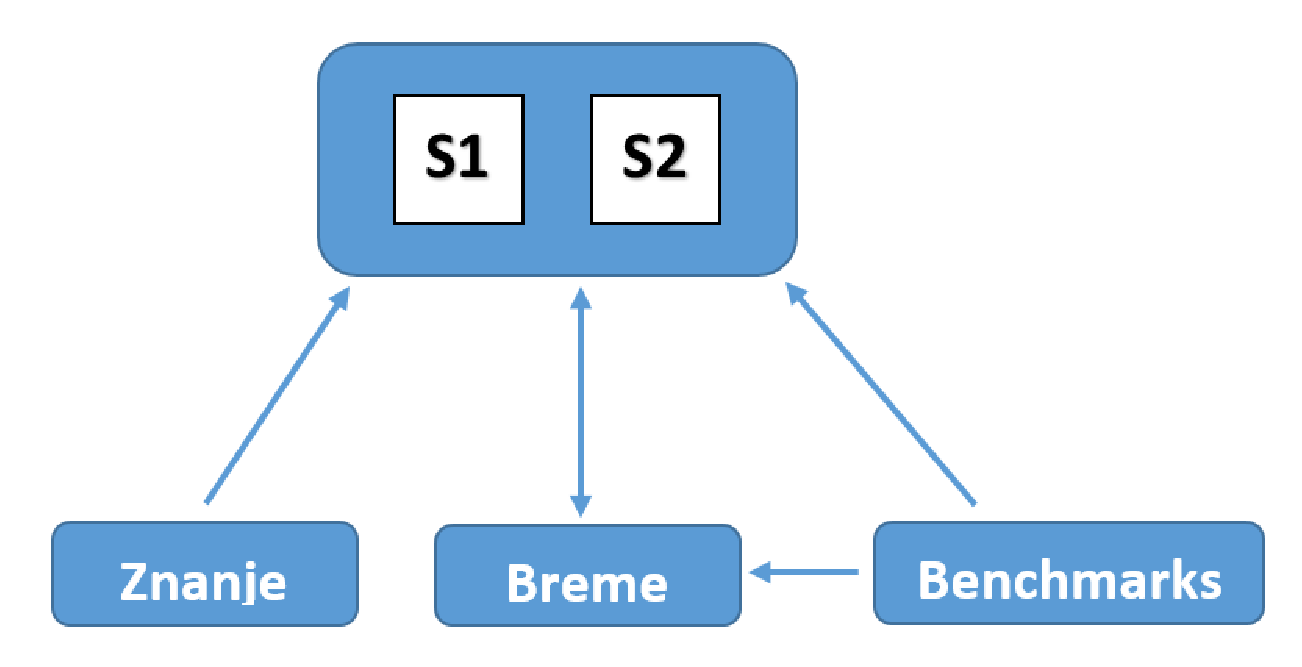
\includegraphics[scale=0.5]
{4_vzorec.eps}}
\caption{Odvisnost izbire S1 in S2 glede na podane atribute.}
\label{fig:miselni}
\end{figure}

\subsection{Izbira ciljnih sistemov}

Za ciljni sistem bi lahko izbrali kak�nega od ve�jih ponudnikov obla�nih storitev kot so Google Cloud, Amazon web service, Microsoft Azure, lahko tudi kak�nega manj�ega, naprimer Rackspace. Ve�ina teh ponudnikov ima omejene zastonjska testna obdobja, med katerimi bi lahko izvedli meritve.
Ker imamo dostop do ra�unalnika Raspberry Pi \footnote{http://www.raspberrypi.org/} in predvsem zastonjskih verzij obla�nih storitev, nas zanima primerjava med temi platformami. Raspberry Pi je ra�unalnik, ki stane okrog 30 evrov in ne porabi prakti�no ni� elektrike, v zameno pa ponuja primerno majhno zmogljivost. Nepla�ljive obla�ne storitve so mo�no �asovno omejene ali pa ponujajo prav tako zelo majhne zmogljivosti.
Zaradi na�ih predznanj lahko storitev za stre�nik, katerega ustroj in delovanje poznamo, bolje optimiziramo, kot obla�no storitev, kar je prav tako vredno preveriti.

Ker pa je implementacija optimizirane storitve in postavitev lastne gru�e relativno zahtevno opravilo, mi pa imamo na voljo omejen �as, smo se odlo�ili za testiranje zmogljivosti gru�e ra�unalnikov Raspberry Pi. Le ti so se v zadnjem �asu zaradi nizke cene na mnogih podro�jih ra�unalni�tva za�eli uporabljati. Nas zanima, ali so ra�unalniki tak�nega tipa primerni tudi za uporabo na podro�jih, ki zahtevajo ra�unsko mo�. Na podlagi izmerjenih rezultatov lahko primerjamo zmogljivost z druga�nimi sistemi, na katerih so meritve �e opravljene. Prav tako lahko nadaljujemo raziskovanje na tem podro�ju z poskusom optimizacije enake storitve na druga�nem sistemu opravimo v prihodnosti.

\subsection{Breme in cilj primerjave}

Za storitev, ki jo bo na�a gru�a ponujala, smo izbrali manipulacijo nad frekven�nim spektrom avdio datotek. To pomeni, da smo implementirali porazdeljen algoritem FFT, ki pretvori datoteko iz vzor�nega prostora v frekve�ni spekter, nato nad temopravimo preprosto operacijo naprimer zamik v vi�je frekvence, nato pa z inverznim FFT naredimo spet datoteko v vzor�nem prostoru.

Bremena so tako razli�no velike zvo�ne datoteke. Ker na� spletni stre�nik, ki to storitev ponuja, sprejme eno ali ve� datotek, testiramo tudi izvajanje ve�ih instanc algoritma hkrati.

Cilj primerjave je ugotoviti, ali je ra�unalnik Raspberry Pi primeren za postavitev gru�e, ki bo izvajala ra�unsko zahtevne storitve. Da bi to ugotovili, moramo primerjati �as izvajanja na procesorju, �as latence oddaljenega sistema prek medmre�ja in �as po�iljanja podatkov po gru�i.

\section{Sistem}

Na� sistem je gru�a ra�unalnikov, narejena po vzoru Beowulf gru�. Namenjena je zaganjanju porazdeljenih programov. Trenutno sta v mre�o povezana dva ra�unalnika Raspberry Pi, model 1B in model 1B+. Povezani so v gru�o s pomo�jo knji�njice MPI. Do njega imamo SSH dostop tudi z zunanjega omre�ja. Storitev je dostopna prek stre�nika, ki smo ga implementirali sami.

\begin{figure}[H]
\centerline{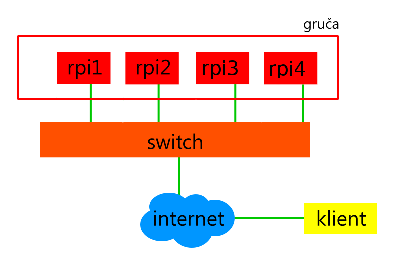
\includegraphics[scale=1.5]
{4_shemaSistema.eps}}
\caption{Shema sistema. Rde�i kvadrati so ra�unalniki Raspberry Pi, bledo rde�ih ni.}
\label{fig:gruca}
\end{figure}

Do tega sistema dostopamo s klienti, ki so izven lokalnega omre�ja. Gru�o uporabljamo kot ra�unski stre�nik, ki po zahtevi klienta izvaja porazdeljeno hitro Fourierjevo transformacijo. Klient prek omre�ja po�lje podatke v obliki glasbene datoteke, gru�a pa podatke sprejme (to stori stre�nik, ki te�e na master ra�unalniku gru�e) in izvajanje algoritma porazdeli prek vseh ra�unalnikov v gru�i, vklju�no s sabo.

V za�etku smo testirali dostop do gru�e od zunaj in delovanje sistema MPI na ra�unalniku rpi1. To smo storili tako, da smo na njem poganjali z MPI implementiran algoritem porazdeljeni Quicksort (porazdeljeno hitro urejanje\footnote{http://en.wikipedia.org/wiki/Quicksort\#Parallelization}).

Pri povezovanju Raspberry Pi-jev v gru�o smo uporabili Message Passing Interface(MPI), ki je standard za izmenjevanje sporo�il med ra�unalniki oz. procesih v ve�-ra�unalni�kih sistemih, gru�ah in delovnih postajah. Omogo�a komunikacijo to�ka-to�ka, skupinske komunikacije, spremljanje delovanja in tudi spreminjanje topologije za posamezen program. MPI je standard, ki omogo�a velik nabor funkcij, vendar za uporabo standarda ni potrebno poznati vseh. Pri sami komunikaciji ra�unalniki med seboj uporabljajo implementacijo MPICH2 \cite{4Mpich},
ki je zelo raz�irjena programska knji�nica poleg tega pa je enostavna za vzpostavitev in uporabo. Na vsakem ra�unalniku je implementacija 
MPICH2 in datoteka (machinefile)\cite{4Gruca} v kateri so zapisani IP naslovi sodelojo�ih(sosednjih) lokalnih ra�unalnikov, na katere se delo porazdeli.

Implementirali smo porazdeljeni algoritem FFT, ki se izvaja na gru�i. 

\subsection{Implementacija storitve}

V gru�o smo dodali ve� ra�unalnikov, da je prava gru�a, ne le en ra�unalnik, na katerem te�e MPI. Raspberry Pi smo pripravili na delovanje v gru�i tako, da smo klonirali sliko datote�nega sistema. Potrebni so bili popravki v konfiguraciji omre�ja in sprememba hostname-a vsakega ra�unalnika. Po tem gru�a deluje brez te�av.

Implementirali smo storitev, ki zvo�no datoteko pretvori v binarno s pomo�jo knji�njice \texttt{libsndfile}\cite{4Audio}. Testiranje smo izvedli z zvo�no datoteko, veliko pribli�no 8 miljonov vzorcev (okrog 3 minute zvoka). Program na enem jedru te�e zelo po�asi. Ni se izpolnil strah, da bi algoritem tekel prehitro, da bi se ga izpla�alo poganjati na gru�i. Imeli smo nekaj te�av s kodiranjem datoteke nazaj v zvo�no datoteko.

Pretvorbo izvajamo z rekurzivnim algoritmom FFT. Implementacija je zaradi uporabe razreda ValArray iz knji�njice STL po�asna, �e je prevanjanje izvedeno z Microsoft Visual Studio prevajalnikom. Program, ki se izvaja na gru�i, na kateri te�e Linux (distribucija Arch Linux), je preveden s prevajalnikov gcc, ki se v tem primeru obna�a veliko bolje - koda se izvaja hitreje.

\vspace{10pt}

Implementirali smo stre�nik, ki sprejema zahtevke z eno ali ve� datotekami in nato odgovori. Implementirali smo tudi klienta, ki po�ilja zahtevek z eno ali ve� datotekami in sprejme odgovor stre�nika.

Program, ki izvaja manipulacije frekven�nega spektra, upo�teva lastnosti hitre Fourierjeve transformacije in pravilno obdeluje zvok. Zavr�emo del frekven�nega spektra, ki je zrcalna slika relevantnega dela. Transformacije, ki jih izvajamo na preostanku, so zato bolj smiselne in se obna�ajo kot pri�akovano.

\vspace{10pt}

% povezovanje v enoten sistem

\section{Meritve}

Na� problem predstavlja veliko ra�unsko breme gru�i ampak relativno majhno breme za prenos podatkov prek omre�ja. Na enem vozli��u traja obdelovanje 5 sekund zvoka okrog 40 sekund. Algoritem je hitrostnega razreda $O(n * log(n))$.

Zaradi tipa problema in bremena nas zanimajo �asi ra�unanja (procesiranja na gru�i, wall-clock time, v odvisnosti od �tevila uporabljenih vozli�� in velikosti bremena), prenosa podatkov na in iz gru�e (latenca omre�ja - �as prenosa je najbr� zanemarljiv, saj so datoteke velike med 1MB in 10MB), latence prenosa podatkov med vozli��i v gru�i (da vidimo, ali je paralelizacija na gru�i primerna ali bi bilo bolje uporabljati paralelizacijo na ve� jedrih ali podobni arhitekturi) in najve�je �tevilo datotek, ki jih lahko obdeluje hkrati, preden se gru�a ali deli nje sesujejo.

Mertive smo izvedli na 1, 2 in 4 ra�unalnikih v gru�i. Izvedli smo teste z enim 5, 20, 60 in 180 sekund dolgo vhodno zvo�no datoteko in z 1, 5, 10 in 200 vhodnimi datotekami velikosti 5 sekund. Test 200 datotek po 5 sekund je namenjen temu, da gru�i zmanjka spomina in se sesuje.

Vse teste smo ponovili trikrat.  

\subsection{Izmerjeni �asi: razli�no velike datoteke}

\begin{table}[h]
\begin{tabular}{l|cccc}
RPIs & n[s] = 1  & n[s] = 5  & n[s] = 20  & n[s] = 60  & n[s] = 180 \\ \cline{1-6}
1    & 6,36      &    21,85  &    86,11   &   359,54               \\
     & 6,23      &    20,70  &    85,98   &   361,90               \\
     & 6,48      &    21,73  &    84,97   &   363,97               \\ \cline{1-6}
2    & 5,27      &    14,50  &    44,69   &   179,31               \\
     & 5,23      &    14,08  &    48,99   &   179,84               \\
     & 5,20      &    13,08  &    48,35   &   178,99               \\ \cline{1-6}
4    & 8,26      &    10,67  &    27,85   &    94,49   &    193,99  \\
     & 9,31      &    10,66  &    28,50   &    93,18   &    203,01  \\
     & 9,34      &    11,06  &    27,15   &    97,29   &    201,75  \\
\end{tabular}
\end{table}

\begin{table}[h]
\begin{tabular}{l|cccc}
RPIs & N[f] = 1  & N[f] = 5   & N[f] = 10  & N[f] = 200  \\ \cline{1-5}
1    & 21,85     & 102,38     & 208,68                   \\
     & 20,70     & 104,35     & 203,89                   \\
     & 21,73     & 103,75     & 218,35                   \\ \cline{1-5}
2    & 14,50     &  70,95     & 126,58                   \\
     & 14,08     &  70,32     & 150,61                   \\
     & 13,08     &  71,55     & 129,25                   \\ \cline{1-5}
4    & 10,67     &  55,44     &  98,99                   \\
     & 10,66     &  55,93     &  95,94                   \\
     & 11,06     &  55,80     &  95,94                   \\
\end{tabular}
\end{table}

Razlika med 2 in 3 vozli��i je premajhna, da bi lahko sklepali na pohitritev. Zaradi tipa algoritma (FFT se rekurzivno deli vedno na dva dela, zato deluje dobro le, �e uporabljamo $2^n$ paralelnih niti.

Ker za dovolj velik $n$ velja $n*log(n) > n*log(n/m)*m$, je hitrost re�evanja problem ve�ja, �e re�ujemo ve� manj�ih problem, kot enega velikega. To je razlog, da ne porazdeljujemo po gru�i po drevesu razcepa podatkov, ki ga izvaja FFT, ampak razdelimo vse podatke na $m$ delov in nato odbelujemo vsakega posebej, pri �emer je $m$ �tevilo ra�unalnikov v gru�i. To je slaba re�itev za zelo velik $m$ ali zelo majhne zahtevke, saj bi se lahko poznala izguba kvalitete zvoka, ki jo to prinese. Razlika se na normalnih zahtevkih in na�em $m$ sicer ne pozna. Tak�en pristop se uporablja tudi v praksi, predvsem kadar se izvaja transformacije v realnem �asu (sproti).

 % 1.Poglavje

\backmatter
%\include{glossary}
%\include{notat}
\bibliographystyle{ieeetr} %The style you want to use for references.
\bibliography{mro} %The files containing all the articles and books you ever referenced.
\printindex %Make an index AUTOMATICALLY

\end{document} 
